\chapter{Methodology}
\label{chap:met}

This section provides a comprehensive overview of the software requirements and methods employed in this thesis. Section \ref{meth:req} outlines the essential requirements that were established at the outset of the study, emphasizing that their fulfillment is essential for the successful completion of the thesis. Additionally, we discuss the inclusion of supplementary requirements, which are not mandatory but offer potential for the integration of additional features. In Section \ref{meth:design}, we delve into the design choices made for the application, elaborating on the underlying decisions that influenced its development. Section \ref{meth:modules} provides a concise overview of the various modules comprising the application.

\section{Software Requirements}
\label{meth:req}
The goal of this thesis is to create an application that will allow developers to quickly and easily understand and navigate Rust source code. The purpose of the application is to provide developers with a lightweight, HTML-based report of a project that contains all of the essential features and information they need to efficiently and effectively develop software using Rust programming language. The report should be designed to be both informative and engaging, with clear, concise information about the project and its components. The report should also be easy to use, with intuitive navigation features that make it easy for developers to access and understand the information it provides. By creating a report that combines the best features of IDE's, this application will help to improve development process and make it easier and faster to work with Rust projects.


% TODO: MUST/DONE/ ??
We have opted to partition the project requirements into two distinct tables, namely "Obligatory" and "Additional" requirements. Table \ref{table:must_req} delineates the set of requirements that are deemed mandatory for the successful completion of the project:

% \begin{longtable}{c|c}
% \caption[Requirements for the project]{Project requirements} \label{table:req} \\
% \hline
% Feature & Description  \\
% \hline
% \endhead
% \hline
%  Project tree & The report should provide a comprehensive project tree that displays the structure of the project, including all of the files and folders within the project. This tree view should allow developers to easily navigate the project and understand its structure \\
%  \hline
% \end{longtable}

\begin{longtable}{|p{1.5in}|p{4in}|}
\caption[Obligatory requirements]{Obligatory requirements}\label{table:must_req}\hline
Feature name & Description\\\hline
1. The report &
The application should scan the project directory and generate a comprehensive HTML file, referred to as the "report". The report should provide an overview of the project, including a tree view of the project folders and files.\\\hline

2. Portability & The report must be a single file that works on all popular web browsers. It should be optimized for web use with fast loading times and responsive design for various screen sizes. \\\hline

3. Related files & The application should have the ability to ignore certain files and directories, such as binary files, build directories, static images which are not relevant to the development process. This will ensure that the report is clean and easy to read, only displaying relevant information. \\\hline

4. File content & By clicking on a filename in the project tree, the report should display the content of that file. This will allow developers to quickly access the source code and view it in a clean, formatted manner. \\\hline

5. Highlight & The content of the report should be highlighted, easy-to-read manner, with the lines in the file number for reference. This will make it easier for developers to navigate the code and understand its structure. \\\hline

6. Hover information & When hovering the cursor over a token, the report should provide additional information about it, including the signature of the function or the type of variable, the path of its declaration, and any associated doc strings. This will make it easier for developers to understand the code and its functionality. \\\hline

7. Navigation menu & By clicking on a token, the report should open a navigation menu that displays information about the definition and references of the token. The navigation menu should have two tabs: Definition and References. The Definition tab should be open by default and contain links to the file and line number of the struct, function, or module definition. The References tab should contain links to the file and line number of all struct, function, or module usage, making it easy for developers to find and understand references to the token. \\\hline

8. Return to original location & The report must allow developers to easily return to the place where they began a navigation jump. This feature will enable developers to quickly move between different parts of a project without losing their place or becoming disoriented. \\\hline

9. Hiding block expressions & The application must provide the ability to hide and show large blocks of code, such as functions, modules, or other block expressions \cite{rust-book-code-blocks}, for improved code readability. This feature will enable developers to focus on specific areas of code without being overwhelmed by the complexity of the entire project.\\\hline 

10. User-friendly interface & The report should be intuitive and user-friendly, with a clear structure, and be similar to modern IDEs. This will improve the overall development process and make it easier for developers to work with Rust programs.\\\hline

\end{longtable}

Table \ref{table:could_req} describes requirements that could be done or could be considered as direction for further work.

\begin{longtable}{|p{1.5in}|p{4in}|}
\caption[Additional requirements]{Additional requirements}\label{table:could_req}\\\hline
Feature name & Description\\\hline
1. Customizable style themes & The report should provide developers with the ability to customize the style theme dynamically using pre-set style themes. This will help to improve the overall usability and accessibility. \\\hline

2. Project search & The report must include a robust code search feature that allows developers to quickly search for specific symbols within the whole scanned project.\\\hline

3. Errors & The application must generate a report even if the project contains syntax errors or warnings. The report should clearly indicate the location and type of errors or warnings, and provide suggestions or solutions to fix them. \\\hline

\end{longtable}



\section{Design}
\label{meth:design}
\begin{figure}[ht]
\centering
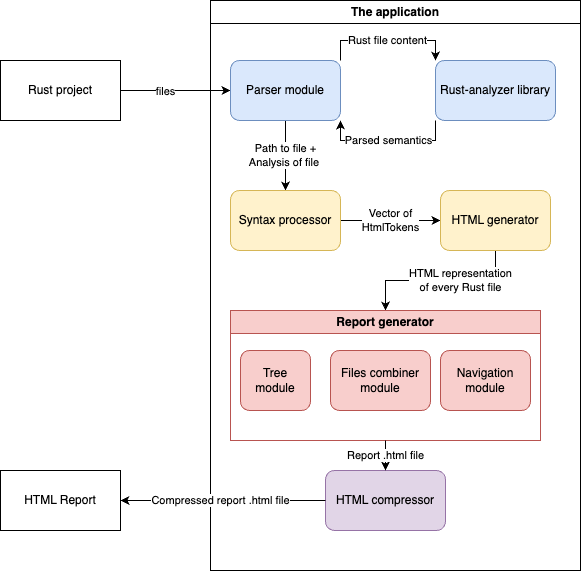
\includegraphics[width=15cm]{figs/thesis_flow3.png}
\caption{Architecture of the HTML generation process}
\label{fig:flow}
\end{figure}


This section describes the architecture of the HTML report generation application for Rust projects. It provides a detailed explanation of the steps taken to develop the application, including the technologies used, the algorithms designed, and the challenges faced during the development process.

The design chapter of the HTML report generation application aims to outline the various modules and their interconnectedness that facilitate the generation of a single HTML report file. The process of software development is a complex task that requires a deep understanding of the codebase, especially when working with code written by different people and lacking in documentation. To address this problem, developers have increasingly turned to special programs and tools that make comprehending and writing code more convenient. Among these approaches, text program visualization has emerged as the most popular and useful method, employed in most Integrated Development Environments (IDE), code viewers, and documentation generators.

The HTML report generation application adopts a modular approach, consisting of several interconnected modules that work together to produce a single HTML report file. The flow of data through the application starts with the Parser module, which scans the Rust project directory and receives all the files. Each file is then sent to the Rust-analyzer library, which generates a semantics object for every source file and an analysis object for the entire project. The Parser module builds analysis of file, which is passed to the Syntax processor. The Syntax processor evaluates analysis of file, and generates a vector of HTML tokens for each file. These vectors are then forwarded to the HTML generator, which combines them into an HTML representation of one file. The resulting file is then sent to the Report generator.

The Report generator comprises three interconnected modules: the Tree module, the Files combiner module, and the Navigation module. The Tree module generates a tree structure of the Rust project, which acts as an overview of the entire codebase. The Files combiner module combines all the HTML representations of individual files generated by the HTML generator into a single file. The Navigation module provides additional functionality to the report, such as code jumping to functions and definitions and displaying information about variables when the user's cursor hovers over them. Once all the modules have performed their tasks, the report is sent to the HTML compressor, which compresses the HTML to decrease the size of the final report.

To implement this design, which can be viewed as a diagram in Fig.\ref{fig:flow}, the application was developed using the Rust programming language and several external libraries, including Rust-analyzer \cite{crates-rust-analyzer}, Syn \cite{crates-syn}, Tera \cite{tera-official} and minify \cite{minify-github}. The modular design of the application allows for easy customization and extension, ensuring that the application remains flexible and adaptable to meet the evolving needs of Rust developers. The application also features a user-friendly interface that allows users to specify the location of the Rust project directory, output format, and compression level for the HTML report. The end result is an efficient and intuitive application that streamlines the process of code comprehension and makes Rust development more convenient and productive.

% To improve the readability of the HTML report, we added CSS styling. We designed the CSS to make the code more visually appealing and easier to read by using color-coding, font styles, and other design elements.

% Finally, we compiled the resulting binary file for Linux x86 to ensure that the project is easily accessible to all developers. The launch of the binary file can be customized via command-line arguments, allowing users to adjust the application's behavior as needed.

% Overall, our goal in designing the application was to provide developers with a powerful tool that is both intuitive and user-friendly. By combining the strengths of Rust and rust-analyzer with modern web design principles, we believe that our application will provide developers with a new level of efficiency and ease of use when working with Rust code.


\section{Overview of Modules}
\label{meth:modules}
This section provides a comprehensive description of the modules that have been developed as part of the HTML report generation tool for Rust programming language. Specifically, it includes a detailed description of the parser \ref{chap:modules:parser}, Syntax processor \ref{chap:modules:processor}, HTML generator \ref{chap:modules:generator}, report generator \ref{chap:modules:report_generator}, and compressor modules.

\subsection{Parser Module}
\label{chap:modules:parser}

These sections describe possible approaches to code parsing, their compatibility with the project, and the challenges faced during the implementation of the parser module.

Parsing code accurately is a crucial task in the domain of static analysis. Several approaches exist for performing this task, with varying degrees of complexity and effectiveness.

% There are several possible solutions to the challenge of code parsing, each with its own benefits and drawbacks. One option is to use the Rust compiler, which is open-source and available on GitHub \cite{rust-github}. The primary advantage of this solution is the closeness of the parsing results to the current state of the project, since the same code is used for both project compilation and parsing. However, while the Rust compiler's output can be highly accurate, the codebase is quite extensive and the API for obtaining static information about the code is not very user-friendly.

% Rust-analyzer is a compiler frontend library specifically designed for Rust. It provides a convenient and well-designed API for extracting information about the codebase's abstract syntax tree (AST). The rust-analyzer library is optimized for parsing large codebases, and it does not involve compiling the code, making it a more efficient choice for our project. Additionally, the library is modular and easy to use, making it a good fit for our needs. By using rust-analyzer, we were able to extract detailed information about the codebase's syntax, including information about tokens, types, and range, as well as information about definitions and references. This information is used to create an array of structs for generating the HTML report.


%%%%%

One approach involves building a custom parsing solution from scratch, which essentially involves implementing the initial stages of a compiler, including lexical analysis, syntactic parsing, and semantic analysis. While this approach may be necessary in some situations where a suitable solution is required, it can be a time-consuming and effort-intensive process, particularly in complex projects. Thus, it turned out to be unsuitable for the present project.

Another approach involves using existing compiler tools, which are open-source and available on GitHub \cite{rust-github}, to extract the necessary information. As the parsing of code is the first step in the compilation process, the compiler already possesses this information. Extracted compilation information is exactly what is required for our Parser module. The primary advantage of this solution is the closeness of the parsing results to the current state of the target project since the same code is used for both project compilation and parsing. Initially, this approach was chosen for the project. However, several difficulties were encountered during its implementation. For instance, the Rust compiler is a large and unwieldy project, making it challenging to extract intermediate compilation results from it. Moreover, it proved problematic to obtain cross-entity relations necessary for comprehending where functions and variables were declared. Additionally, this approach is unable to produce information in cases where the code was written with compile errors. Consequently, this approach was abandoned in favor of a different solution.

The third approach, which was ultimately adopted in this project, involves utilizing a third-party solution to analyze Rust source code. In particular, the Rust-analyzer \cite{crates-rust-analyzer} project was chosen for its open-source implementation of the Language Server Protocol \cite{lsp} for the Visual Studio Code IDE. Additionally, the Rust-analyzer provides a Rust library API that allows users to analyze Rust codebases comprehensively, including parsed AST (Abstract Syntax Tree), cross-entity relations, and searching for references, among other features related to IDE. This approach aligns well with the present project's requirements and provides all the necessary information to implement all visualization features. However, usage of Rust-analyzer tool also has several drawbacks, such as long loading times due to indexing all dependencies and a lack of API documentation. Nevertheless, the utilization of the Rust-analyzer for the parsing module is the most optimal solution available. By using Rust-analyzer, we were able to extract detailed information about the codebase's syntax, including information about tokens, types, and ranges, as well as information about definitions and references. This data are passed to the Syntax processor module \ref{chap:modules:processor}.

Overall, the Rust-analyzer library was the best choice for our project, as it provides user-friendly API and was designed specifically for parsing Rust code. Its modular and efficient design allowed us to extract the necessary information from the codebase quickly and accurately, and it ultimately helped us to create a powerful and efficient tool for navigating and understanding Rust code.

\subsection{Syntax processor}
\label{chap:modules:processor}
The primary objective of the Syntax processor module is to extract relevant information from Rust-analyzer about one source file and generate a vector of HtmlToken objects. These tokens encapsulate data pertaining to syntax highlighting, hover functionality, and navigation information. It is crucial to emphasize that the processor does not directly render HTML content; rather, it focuses on processing the output of Rust-analyzer and aggregating it into a convenient data structure for next modules.

A more comprehensive elucidation of this module will be expounded upon in Section \ref{chap:impl:processor}.


\subsection{HTML generator}
\label{chap:modules:generator}

The HTML generator module assumes responsibility for the rendering HTML content for source file. Its primary function entails transforming the conveniently structured representation of a file, as provided by the parser module, into corresponding HTML content for the given file. The rendering process occurs in two distinct steps, each serving a specific purpose.

Firstly, the module generates a vector of Line structures. Each Line structure contains essential information such as the line number, the rendered HTML content of the line, and collapse information. The inclusion of collapse information serves the purpose of fulfilling the requirement outlined in Table \ref{table:must_req}, which pertains to the implementation of hiding block expressions.

Secondly, the generated vector of Line structures is passed to the Tera template engine \cite{tera-official}, which serves as a Rust-based alternative to the widely used Jinja library \cite{jinja-official}. Tera template handles the appropriate placement of line contents and ensures the correct line-collapsing behavior in accordance with the specified requirements.

A more detailed examination of this module will be provided in Section \ref{chap:impl:generator}.

\subsection{Report generator}
\label{chap:modules:report_generator}

The report generator module serves as a central entity responsible for combining and integrating diverse elements, including file content generated by the HTML generator module, tree content derived from the tree module, navigation content, and static CSS files. Similar to the HTML generator module, the report generator leverages the capabilities of Tera templates to facilitate the generation of the final output HTML file.

Further elaboration on the implementation details of the report generator module can be found in Section \ref{chap:impl:report_generator}


\subsection{Compressor}
\label{chap:modules:compressor}
In comparison to other modules, the compressor module serves as a compact component integrated with the Minify Rust crate \cite{minify-github}. Its primary function is to perform a straightforward yet crucial task, which involves diminishing the size of the output file while preserving its content. This is achieved by eliminating redundant spaces and tabs, and shortening JavaScript and CSS segments, among other optimizations.

Regarding quantitative measurements, the incorporation of the compressor module has resulted in a substantial reduction of approximately six times in the number of lines within the final report file, accompanied by a 25\% decrease in file size, as quantified in bytes. This step holds significance in relation to the Portability feature outlined in the requirements, as depicted in Table \ref{table:must_req}.

\section{Conclusion}
In this chapter, we provided functional requirements and an overview of the various modules developed as part of the HTML report generation tool for the Rust programming language. These modules include the parser, Syntax processor, HTML generator, report generator, and compressor.

The parser module plays a critical role in accurately parsing the code and extracting essential information for static analysis. We explored different approaches to code parsing, including building a custom solution, utilizing existing compiler tools, and leveraging third-party solutions. After careful consideration, we selected the Rust-analyzer as the most suitable option, as it offers a well-designed API and comprehensive analysis capabilities. The integration of the Rust-analyzer facilitated the extraction of detailed syntax information, such as tokens, types, and ranges, enabling the creation of a data structure that serves as input for the Syntax processor module.

The Syntax processor module focuses on processing the output of the Rust-analyzer and aggregating relevant information into HtmlToken objects. These objects encapsulate data related to syntax highlighting, hover functionality, and navigation, providing a convenient data structure for subsequent modules.

The HTML generator module transforms the structured representation of a source file, generated by the parser module, into corresponding HTML content. It involves generating Line structures and utilizing the Tera template engine for rendering HTML and implementing line-collapsing functionality.

The report generator module acts as a central entity that combines file content, tree content, navigation information, and static files to generate the final output HTML file. It employs Tera templates for the effective generation and integration of these elements.

Finally, the compressor module, integrated with the Minify Rust crate, plays a crucial role in reducing the size of the output file while preserving its content. By removing unnecessary spaces, and tabs, and shortening JavaScript and CSS segments, significantly reduces the number of lines and file size, enhancing the portability of the generated HTML report.

In conclusion, the design and implementation of these modules have contributed to the development of a powerful and efficient HTML read-only IDE for the Rust programming language. The careful selection of tools and the integration of optimization techniques have resulted in a tool that facilitates code comprehension, navigation, and analysis, ultimately enhancing the development workflow for Rust programmers.


